\subsection{Studienergebnisse}
\label{sec:study_results_quantitativ}

Im Folgenden werden die Ergebnisse der beschriebenen Case-Study vorgestellt. Nach einem Überblick über die Studienteilnehmer werden die Einflusshypothesen durch Störgrößen außerhalb von Erklärungen analysiert. Darauf folgend werden die abstrakten Hypothesen (siehe \autoref{sec:evaluation_hypothesis}) jeweils auf die in \autoref{sec:explanation_requirements} vorgestellten Anforderungen übertragen und im Anschluss geprüft. Für die Überprüfung der Hypothesen wird jeweils die Wahrscheinlichkeit $ p $ berechnet, dass ein Unterschied der Daten nur zufällig zustande gekommen ist. Für alle Wahrscheinlichkeiten wird für $ p < 0.05 $ angenommen, dass ein signifikanter Unterschied zwischen zwei Bedingungen vorliegt \cite[vgl.][]{wohlin2012experimentation}.

\subsubsection{Übersicht}

Im Zeitraum der Studie haben insgesamt 9~745 \textit{End User} Daten, welche die benötigten Metriken enthalten, beigetragen. Dabei sind diese 41~540 Routen gefahren. Dies enthält allerdings auch Daten, von \textit{End Usern}, die keine aktive Navigation durchgeführt haben. Um diese Daten herauszufiltern, wurden Routen, bei denen weniger als 5 Kilometer zurückgelegt wurden, nicht berücksichtigt. Schlussendlich sind im zur Analyse verwendeten Datensatz folglich 4~012 \textit{End User} mit 16~531 gefahrenen Routen enthalten. Für 625 der Routen liegt darüber hinaus eine Bewertung durch \textit{End User} vor (siehe \autoref{tab:study_user_group_overview}).

Die Studienteilnehmer der Gruppen 3 und 4 erhalten während der Navigation so lange keine Erklärung, wie auf der aktuellen Route keine besonderen Vorkommnisse auftreten. Dies ist der Fall, wenn das Verkehrsaufkommen \glqq normal\grqq{} ist und die \textit{End User} während der gesamten Fahrt guten GPS-Empfang haben (siehe \autoref{sec:traffic_volume_definition} und \autoref{sec:gps_accuracy_definition}). Bei der Betrachtung von einzelnen Routen werden die Teilnehmer folglich in die Gruppen 1 oder 2 umsortiert, falls sie während der Navigation keine Erklärung erhalten haben. Bei der Betrachtung von Metriken über mehrere Routen werden Teilnehmer den entsprechenden Gruppen zugeordnet, wenn NUNAV ihnen mindestens einmal eine Erklärung aus der Studiengruppe angezeigt hat. Eine Übersicht findet sich in \autoref{tab:study_user_group_overview}.

\begin{table}[b!]
    \centering
    \begin{tabular}{p{.26\textwidth} c c c}
        \hline
        \multirow{2}{*}{Studiengruppe} & \multirow{2}{*}{Anzahl der Nutzer} & \multicolumn{2}{c}{Anzahl der Routen} \\
        & & Insgesamt & Mit Nutzerbewertung \\
        \toprule
        Gruppe 1            & 1 778 & 4 807  & 133 \\
        Gruppe 2            & 1 397 & 3 413  & 135 \\
        Gruppe 3            & 468   & 4 571  & 184 \\
        Gruppe 4            & 369   & 3 740  & 173 \\
        \midrule
        Insgesamt           & 4 012 & 16 531 & 625 \\ 
        \toprule
    \end{tabular}
    \caption{Übersicht über die Daten der Studiengruppen}
    \label{tab:study_user_group_overview}
\end{table}

\subsubsection{Einflüsse außerhalb von Erklärungen}
\label{sec:evaluation_other_dependencies}

Zunächst wird die Hypothese geprüft, dass eine schlecht vorausgesagte Ankunftszeit (\textit{Estimated Time of Arrival (ETA)}) im Vergleich zur wirklichen Ankunftszeit (\textit{Actual Time of Arrival (ATA)}) einen negativen Effekt auf die Anzahl der Abweichungen von der Route sowie die Zufriedenheit mit der Route hat. Die gleichen Auswirkungen werden für ein häufiges Auftreten von Positionsungenauigkeiten bei der Navigation untersucht. Dies wird analysiert, da ein negativer Zusammenhang vermutet wird, der die Ergebnisse der Untersuchung beeinflussen könnte. Überprüft werden die folgenden Hypothesen innerhalb der Kontrollgruppe (Gruppe 1: Ohne Erklärungen):

\begin{enumerate}
    \item[1.1] WENN die \textit{ATA} mehr als 10 \% und mindestens 2 Minuten von der \textit{ETA} abweicht, DANN hat dies einen signifikant messbaren negativen Einfluss auf die Zufriedenheit der Nutzer mit der Route.
    \item[1.2] WENN die \textit{ATA} mehr als 10 \% und mindestens 2 Minuten von der \textit{ETA} abweicht, DANN ist die Anzahl der Routenabweichungen signifikant messbar höher.
    \item[1.3] WENN \textit{NUNAV Navigation} auf der betrachteten Route pro 5 km durchschnittlich mindestens eine Positionsungenauigkeit aufwies, DANN hat dies einen signifikant messbaren negativen Einfluss auf die Zufriedenheit der Nutzer mit der Route.
    \item[1.4] WENN \textit{NUNAV Navigation} auf der betrachteten Route pro 5 km durchschnittlich mindestens eine Positionsungenauigkeit aufwies, DANN ist die Anzahl der Routen-Abweichungen signifikant messbar höher.
\end{enumerate}

Die statistische Prüfung der Auswirkung von schlecht vorausgesagter Ankunftszeit auf die Anzahl der Routen-Abweichungen erfolgt mittels eines Kruskal-Wallis-Tests. Dieser wird verwendet, da die Datensätze für die beiden Gruppen verschieden lang und nicht normalverteilt (geprüft mit Shapiro-Wilk-Test) und zudem unabhängig voneinander sind. Das Ergebnis zeigt keinen Haupteffekt ($ p = 0.197648 $). Gleiches gilt für die Überprüfung eines Effektes auf die Nutzerzufriedenheit ($ p = 0.564911 $). Folglich können die Hypothesen 1.1 und 1.2 abgelehnt werden.

Für die Überprüfung, ob eine schlechte Positionierung einen Effekt auf die Nutzerzufriedenheit hat, ergibt sich anhand eines Kruskal-Wallis-Test, dass kein signifikanter Effekt vorliegt ($ p = 0.269231 $). Folglich muss Hypothese 1.3 abgelehnt werden. Bei die Prüfung von Hypothese 1.4 kann festgestellt werden, dass die Anzahl der Routen-Abweichungen signifikant höher ist, wenn im Durchschnitt mehr als ein mal pro 5 km eine Positionsungenauigkeit während der Navigation auftritt ($ p = 3.426601e-15 $). Folglich kann Hypothese 1.4 angenommen werden. Da eine häufige ungenaue Positionierung also bereits einen Einfluss auf die Anzahl der Abweichungen von der Route hat, werden Daten mit ungenauer Positionierung bei der Auswertung vom Einfluss von Erklärungen auf die Anzahl der Routen-Abweichungen herausgefiltert.

\subsubsection{Häufigkeit der Nutzung}
\label{sec:06_model_evaluation:usage_analysis}

Bei der Analyse der Nutzungshäufigkeit von NUNAV wurde über den zweiwöchigen Studienzeitrum gemessen, wie viele Routen pro Nutzer und Studiengruppe in diesem Zeitraum gefahren wurden. Für die Überprüfung, ob die Erklärungen die Qualitätsanforderung für eine Erhöhung der Nutzung (NFR1) erfüllen werden folgende Hypothesen aufgestellt:

\begin{enumerate}
    \item[2.1] WENN Teilnehmer Erklärungen erhalten, DANN verwenden sie \textit{NUNAV Navigation} signifikant häufiger, als wenn sie keine erhalten.
    \item[2.2] WENN Teilnehmer nur einen der beiden vorgestellten Erklärungstypen erhalten, DANN nutzen sie \textit{NUNAV Navigation} signifikant seltener, als wenn sie beide Erklärungstypen erhalten.
\end{enumerate}

\begin{figure}[b!]
    \centering
    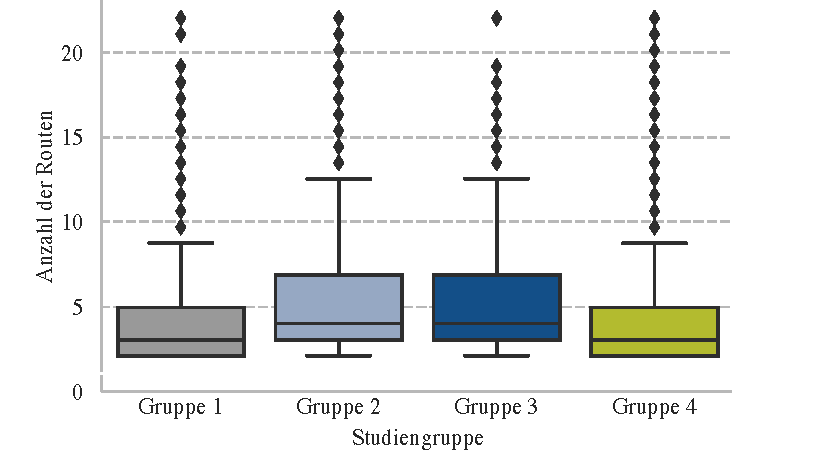
\includegraphics[width=\textwidth]{contents/06_model_evaluation/02_evaluation/res/usage_result_overview.pdf}
    \caption{Anzahl der gefahrenen Routen für jede Studiengruppe}
    \label{fig:evaluation_usage_result_overview}
\end{figure}

\autoref{fig:evaluation_usage_result_overview} enthält eine Übersicht der Verteilung der Anzahl der gefahrenen Routen pro Nutzer für jede Studiengruppe. Für die weitere Analyse werden zunächst Ausreißer herausgefiltert. Dabei werden alle Datenpunkte, welche mehr als dreimal die Standardabweichung vom Median entfernt sind aus dem Datensatz genommen \cite{leyes2013detecting}. Final sind 3~937 Nutzer im Datensatz für die Prüfung der Hypothesen verblieben. Daraus sind die in \autoref{tab:study_usage_results} aufgelisteten Ergebnisse berechnet worden.

Zur Prüfung der Signifikanz wird wieder der Kruskal-Wallis-Test eingesetzt, da auch die Anzahl der gefahrenen Routen pro Studienteilnehmer nicht normalverteilt ist (Shapiro-Wilk: $ p = 0.0 $). Mit $ p = 1.311644e-15 $ als Ergebnis des Kruskal-Wallis-Tests kann davon ausgegangen werden, dass ein Haupteffekt vorliegt.

\begin{table}[htb!]
    \centering
    \begin{tabular}{p{.27\textwidth}p{.27\textwidth}p{.35\textwidth}}
        \hline
        Studiengruppe  & Mittelwert [N] & Standardabweichung [N] \\
        \toprule
        Gruppe 1                & 3.2234 & 3.1688 \\
        Gruppe 2                & 3.1977 & 3.1130 \\
        Gruppe 3                & 4.4225 & 4.2507 \\
        Gruppe 4                & 4.4382 & 3.9367 \\
        \bottomrule
    \end{tabular}
    \caption{Übersicht der Ergebnisse der gefahrenen Routen der Nutzer}
    \label{tab:study_usage_results}
\end{table}

Für die Prüfung zwischen welchen Studiengruppen ein signifikanter Unterschied vorliegt, wird der Dunn-Test \cite{dunn1964multiple} verwendet, welcher die Signifikanz der Unterschiede zwischen den Studiengruppen berechnet. Die Prüfung ergibt, dass jeweils ein signifikanter Effekt zwischen den Gruppen 3 und 4 gegenüber den Gruppen 1 und 2 vorliegt ($ p_{13} = 4.746580e-09 $, $ p_{14} = 7.528428e-09 $, $ p_{23} = 1.977438e-08 $ $ p_{24} = 2.523727e-08 $). Folglich kann abgeleitet werden, dass die Nutzer \textit{NUNAV Navigation} häufiger verwenden, wenn sie \textit{Context}-abhängige Erklärungen erhalten, unabhängig davon, ob diese kombiniert mit den statischen Erklärungen erfolgen. Folglich erfüllen nur die \textit{Context}-abhängigen Erklärungen die Anforderung NFR1.

Die Hypothesen 2.1 und 2.2 müssen allerdings abgelehnt werden, da weder alle Erklärungstypen zu einer signifikant häufigeren Nutzung von NUNAV führen, noch das Bereitstellen beider vorgestellten Typen von Erklärungen zu einer erhöhten Nutzung pro Studienteilnehmer führt im Vergleich zur Präsentation von nur einem der integrierten Erklärungstypen. 

\subsubsection{Nutzerabweichungen von der vorgeschlagenen Route}

Im Folgenden wird die Anforderung NFR2 geprüft, welche fordert, dass die Nutzer weniger häufig von der vorgeschlagenen Route abweichen sollen. Zur Prüfung werden ebenfalls zwei Hypothesen aufgestellt:

\begin{enumerate}
    \item[3.1] WENN der Teilnehmer Erklärungen erhält, DANN folgt er signifikant häufiger der vorgeschlagenen Route als wenn er keine erhält.
    \item[3.2] WENN der Teilnehmer nur einen der beiden vorgestellten Erklärungstypen erhält, DANN folgt er signifikant weniger häufig der vorgeschlagenen Route als wenn ihm beide Arten von Erklärungen präsentiert werden.
\end{enumerate}

\begin{figure}[htb!]
    \centering
    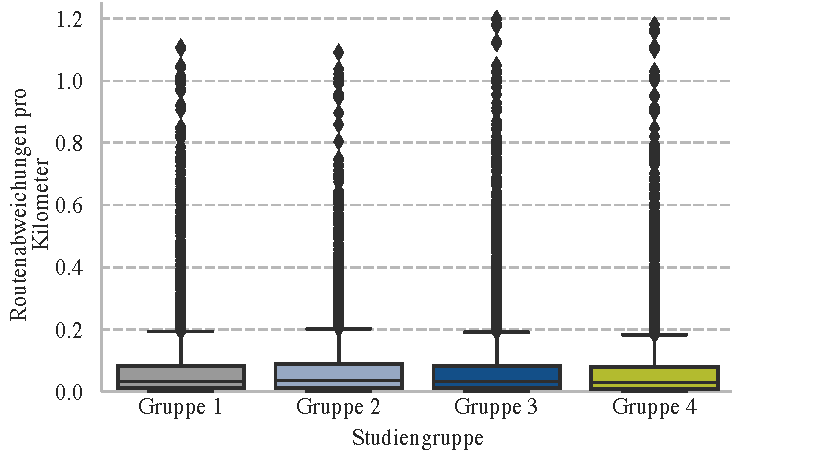
\includegraphics[width=\textwidth]{contents/06_model_evaluation/02_evaluation/res/off_route_result_overview.pdf}
    \caption{Anzahl der Abweichungen von der vorgeschlagenen Route pro Kilometer für jede Studiengruppe}
    \label{fig:evaluation_off_route_result_overview}
\end{figure}

Als Messwert wird die Anzahl der Abweichungen relativ zu Gesamtlänge der Route verwendet. Die Einheit ist Abweichungen pro Kilometer. Zu diesem Messwert, muss erwähnt werden, dass die Erkennung, wann \textit{End User} von der Route abweichen nicht trivial ist. Bei einer wirklichen Abweichung wird dies zum Teil mehrfach gezählt und es kann generell schnell zu falsch positiven Messungen kommen. Aufgrund der großen Datenmenge wird allerdings davon ausgegangen, dass diese Fehler einen vernachlässigbaren Effekt haben. Bei der Betrachtung von Abweichungen von der Route werden außerdem, wie zuvor beschrieben, Navigationen, bei denen es häufig zu einer ungenauen Positionierung kommt aus dem Datensatz herausgefiltert. Außerdem werden auch hier Ausreißer in den Daten mit der gleichen Bedingung herausgefiltert, sodass schlussendlich 16~314 einzelne Navigationen zur Analyse der Routen-Abweichungen im Datensatz verblieben sind. Die Daten für jede Studiengruppe sind in \autoref{fig:evaluation_off_route_result_overview} dargestellt. Die berechneten Ergebnisse sind in \autoref{tab:study_offroute_results} zusammengefasst.

\begin{table}[htb!]
    \centering
    \begin{tabular}{p{.27\textwidth}p{.27\textwidth}p{.35\textwidth}}
        \hline
        Studiengruppe  & Mittelwert [N/km] & Standardabweichung [N/km]\\
        \toprule
        Gruppe 1                & 0.0753 & 0.1293 \\
        Gruppe 2                & 0.0786 & 0.1272 \\
        Gruppe 3                & 0.0803 & 0.1410 \\
        Gruppe 4                & 0.0732 & 0.1328 \\
        \bottomrule
    \end{tabular}
    \caption{Übersicht der Ergebnisse der Routen-Abweichungen pro Kilometer}
    \label{tab:study_offroute_results}
\end{table}

Da auch die Daten der Routenabweichugen nicht normalverteilt sind (Shapiro-Wilk-Test: $ p = 0.0 $), wird zur Signifikanzprüfung der Kruskal-Wallis-Test verwendet \cite{wohlin2012experimentation}. Aufgrund des Ergebnisses von $ p = 0.0000 $, wird abgeleitet, dass ein Haupteffekt vorliegt. Analog zur vorherigen Analyse wird mit dem Dunn-Test die Signifikanz zwischen den einzelnen Studiengruppen geprüft. 

Auch hier wird wieder von einem Signifikanzniveau $ p < 0.05 $ ausgegangen. Folglich weichen die Nutzer der Gruppe 4 signifikant weniger von der vorgeschlagenen Route ab, als die Teilnehmer aller anderen Gruppen ($ p_{14} = 0.0217 $, $ p_{24} = 0.0000 $, $ p_{23} = 0.0029 $). Weitere signifikante Unterschiede gibt es nicht.

Hypothese 3.1 trifft beim Bereitstellen aller Erklärungstypen (Gruppe 4) zu, kann jedoch für die Gruppen 2 und 3 nicht bestätigt werden. Folglich wird diese abgelehnt. Hypothese 3.2 kann angenommen werden, da die Nutzer der Gruppe 4 signifikant weniger von der vorgeschlagenen Route abgewichen sind als die \textit{End User} der Gruppen 2 und 3.

Zusammenfassend kann die Anforderung NFR2 durch das Bereitstellen von allen Erklärungen erfüllt werden. Einzelne Erklärungen weisen keinen signifikant positiven Effekt auf die Anzahl der Abweichungen von der Route auf. Möglich ist folglich, dass die Effekte, der beiden Erklärungstypen nicht reichen. Eine genaue Begründung kann an dieser Stelle allerdings noch nicht gegeben werden.

\subsubsection{Nutzerzufriedenheit mit der aktuellen Route}

Um die Zufriedenheit der Nutzer mit der abgeschlossenen Navigation zu evaluieren, setzt NUNAV auf eine Bewertung mithilfe von 5 Sternen bei Erreichen des Zieles. Dies ist verknüpft mit der Frage \glqq Wie hat dir die Fahrt gefallen?\grqq{} (siehe \autoref{fig:screenshot_destination_reached}). Außerdem sind die Fahrtdauer und zurückgelegte Kilometer angegeben. Die folgenden konkreten Hypothesen werden für die Analyse abgeleitet:

\begin{enumerate}
    \item[4.1] WENN Teilnehmer Erklärungen erhalten, DANN geben sie im Vergleich eine signifikant höhere Bewertung für die Navigation ab, als wenn sie keine Erklärungen erhalten.
    \item[4.2] WENN Teilnehmer nur einen der beiden vorgestellten Erklärungstypen erhalten, DANN geben sie im Vergleich eine signifikant niedrigere Bewertung für die Navigation ab, als wenn sie beide Erklärungstypen erhalten.
\end{enumerate}

\begin{figure}[htb!]
    \centering
    
\includegraphics[width=0.27\textwidth]{contents/06_model_evaluation/02_evaluation/res/rating_screenshot.jpg}
    \caption{Bildschirmfoto des Bewertungsdialogs}
    \label{fig:screenshot_destination_reached}
\end{figure}


Für die Prüfung zwischen welchen Studiengruppen ein signifikanter Unterschied vorliegt, wird ebenfalls der Dunn-Test \cite{dunn1964multiple} verwendet, nachdem ein Kruskal-Wallis-Test einen Haupteffekt zeigt ($ p = 0.00335 $). Daraus resultiert, dass es zwischen den Gruppen 1 und 3 ($ p = 0.005723$) sowie 3 und 4 ($ p = 0.024375 $) einen signifikanten Unterschied bei der Zufriedenheit mit der aktuellen Route gibt.

Mithilfe von \autoref{fig:Rating_Result_Overview} wird abgeleitet, dass es insbesondere mehr 5-Stern-Bewertungen in Gruppe 3 gegenüber den Gruppen 1 und 4 gibt. Die Anteile der ein und zwei Stern Bewertungen unterscheiden sich kaum. Folglich kann gesagt werden, dass die Teilnehmer signifikant zufriedener mit der Navigation sind, wenn sie Erklärungen wie in Gruppe 3 bekommen im Vergleich zu keinen Erklärungen (Gruppe 1) oder allen vorgestellten Erklärungstypen (Gruppe 4).

Da das Geben von Erklärungen die Nutzerzufriedenheit nicht in jedem Fall erhöht, muss Hypothese 4.1 abgelehnt werden. Hypothese 4.2 wird ebenfalls abgelehnt, da es unter anderem einen gegenteiligen Effekt zwischen den Gruppen 3 und 4 gibt.

\begin{figure}[t!]
    \centering
    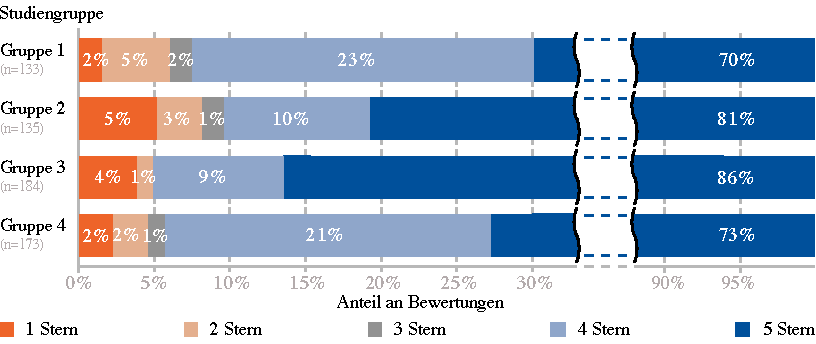
\includegraphics[width=\textwidth]{contents/06_model_evaluation/02_evaluation/res/rating_result_overview.pdf}
    \caption{Verteilung der Teilnehmer-Bewertung der Navigation für jede Studiengruppe bezogen auf die insgesamt abgegebenen Bewertungen}
    \label{fig:Rating_Result_Overview}
\end{figure}

\subsubsection{Zusammenfassung des Einflusses auf die gesetzten Qualitätsziele}

Bei der Analyse der Einflüsse der Erklärungen auf die gesetzten Qualitätsziele für \textit{NUNAV Navigation} müssen die meisten Hypothesen abgelehnt werden. Signifikant negative Einflüsse durch Erklärungen konnten allerdings nicht gemessen werden. Der positive Effekt der integrierten Erklärungen fällt folglich geringer aus, als erwartet. 

Darüber hinaus gibt es einen positiven Effekt durch Erklärungen auf die Nutzung pro Woche und Nutzer, wenn die \textit{End User} \textit{Context}-abhängige Erklärungen erhalten. Sie nutzen NUNAV dann durchschnittlich 4,66 (\textit{Context}-abhängig + statisch) bzw. 4,54 (\textit{Context}-abhängig + statisch) mal pro Woche gegenüber 3,23 (statisch) bzw. 3,27 (keine Erklärung) mal pro Woche.

Die Anzahl der Routenabweichungen wird signifikant positiv beeinflusst (weniger Abweichungen), wenn die \textit{End User} alle Erklärungen angezeigt bekommen (0,073 Abweichungen/km) gegenüber keinen Erklärungen (0,075 Abweichungen/km). 

Außerdem geben die \textit{End User} eine signifikant positivere Bewertung für die Route ab, wenn sie \textit{Context}-abhängige Erklärungen erhalten (durchschnittlich 4,73 Sterne vs. 4,55 Sterne). Hier gibt es allerdings einen negativen Einfluss, wenn die \textit{End User} zusätzlich die statischen Erklärungen erhalten, da diese die Routen dann signifikant schlechter bewerten (durchschnittlich 4,6 Sterne). Eine mögliche Erklärung wäre, dass sich die \textit{End User} Fehler bei der Routenberechnung eher identifizieren können, wenn sie Erklärungen zum Algorithmus erhalten haben. Allerdings kann anhand der Daten keine sichere Begründung gegeben werden.

Folglich erfüllen die \textit{Context}-abhängigen Erklärungen die Qualitätsanforderungen NFR1 sowie NFR3 und tragen somit zu einer signifikant häufigeren Nutzung von \textit{NUNAV Navigation}. Zudem wird die Zufriedenheit der \textit{End User} mit der Navigation signifikant gesteigert. Folglich kann empfohlen werden, diese weiterhin in der Anwendung zu integrieren.

Für die statischen Erklärungen alleine kann kein signifikant positiver Effekt gemessen werden. Jedoch kann ein zusätzlicher, signifikant positiver Effekt im Rahmen von NFR2 gezeigt werden (weniger Routenabweichungen), wenn beide Erklärungstypen angezeigt werden. Allerdings hat diese Kombination der Erklärungen zugleich einen negativen Effekt auf die Routen-Zufriedenheit der \textit{End User}, verglichen mit dem alleinigen Einsatz von \textit{Context}-abhängigen Erklärungen. Für die statischen Erklärungen kann hier folglich keine klare Empfehlung abgeleitet werden.

\newpage